%
% teil3.tex -- Beispiel-File für Teil 3
%
% (c) 2020 Prof Dr Andreas Müller, Hochschule Rapperswil
%
\section{Übertragung mit hilfe der Diskrete Fourier Transformation
\label{reedsolomon:section:dtf}}
\rhead{Umwandlung mit DTF}
Um die Polynominterpolation zu umgehen, gehen wir nun über in die Fourientransformation.
Dies wird weder eine Erklärung der Forientransorfmation, noch ein genauer gebrauch für den Reed-Solomon-Code. 
Dieser Abschnitt zeigt nur wie die Fourientransformation auf Fehler reagiert.
wobei sie dann bei späteren Berchnungen ganz nützlich ist.

\subsection{Diskrete Fourietransformation Zusamenhang
\label{reedsolomon:subsection:dtfzusamenhang}}
Mit hilfe der Fourietransformation werden die \textcolor{blue}{blauen Datenpunkte} transformiert,
zu den \textcolor{darkgreen}{grünen Übertragungspunkten}. 
Durch eine Rücktransformation könnnen die \textcolor{blue}{blauen Datenpunkte} wieder rekonstruiert werden.
Nun zur definition der Diskrete Fourietransformation, diese ist definiert als
\begin{equation}
	\hat{c}_{k} 
	= \frac{1}{N} \sum_{n=0}^{N-1}
	{f}_n \cdot e^{-\frac{2\pi j}{N} \cdot kn}
	,\label{reedsolomon:DFT}
\end{equation}
wenn man nun 
\begin{equation}
	w =
	e^{-\frac{2\pi j}{N} k}
	\label{reedsolomon:DFT_summand}
\end{equation}
ersetzte, und $N$ konstantbleibt, erhält man
\begin{equation}
	\hat{c}_{k}=
	\frac{1}{N}( {f}_0 w^0 + {f}_1 w^1 + {f}_2 w^2 + \dots + {f}_{N-1} w^N)
	\label{reedsolomon:DFT_polynom}
\end{equation}
was überaust ähnlich zu unserem Polynomidee ist.

\subsection{Beispiel
\label{reedsolomon:subsection:Übertragungsabfolge}}
Der Auftrag ist nun 64 Daten zu übertragen und nach 32 Fehler abzusicheren,
16 Fehler erkennen und rekonstruieren.

Dieser Auftrag soll mittels Fouriertransformation bewerkstelligt werden. 
In der Abbildung \ref{reedsolomon:subsection:Übertragungsabfolge} sieht man dies Schritt für schritt,
und hier werden die einzelne Schritte erklärt:
\begin{enumerate}[(1)]
\item Das Signal hat 64 die Daten, Zahlen welche übertragen werden sollen. 
Dabei zusätzlich nach 16 Fehler abgesichert, macht insgesamt 96 Übertragungszahlen.
(siehe Abschnitt \externaldocument{papers/reedsolomon/idee}\ref{reedsolomon:section:Fehlerkorrekturstellen})
Die 32 Fehlerkorrekturstellen werden als Null Übertragen
\item Nun wurde mittels der diskreten Fourientransformation diese 96 codiert.
Das heisst alle Informationen ist in alle Zahlenvorhanden. (Auch die Fehlerkorrekturstellen Null)
\item Nun kommen drei Fehler dazu an den Übertragungsstellen 7, 21 und 75.(die Skala ist Rechts)
Die Fehler können auf den ganzen 96 Übertragungswerten liegen, wie die 75 zeigt.
\item Dieses wird nun Empfangen und mittels inversen diskreten Fourientransormation, wieder rücktransformiert.(Iklusive der Fehler)
\item Nun sieht man den Fehler im Decodieren in den Übertragungsstellen 64 bis 96, da es dort nicht mehr Null ist.
\item Nimmt man nun nur diese Stellen 64 bis 96, dies definieren wir als Syndrom, und transformiert nur dieses Syndrom.
\item Bekommt man die Fehlerstellen wieder, zwar nichtso genau, dennoch erkennt man wo die Fehler stattgefunden haben. 
Dies definieren wir als Locator.
\end{enumerate}
Nun haben wir mit Hilfe der Fourietransformation die 3 Fehlerstellen durch das Syndrom lokalisiert, 
jetzt gilt es nur noch diese zu korrigieren und wir haben unser originales Signal wieder.

\begin{figure}
	\centering
	\resizebox{\textwidth}{!}{
	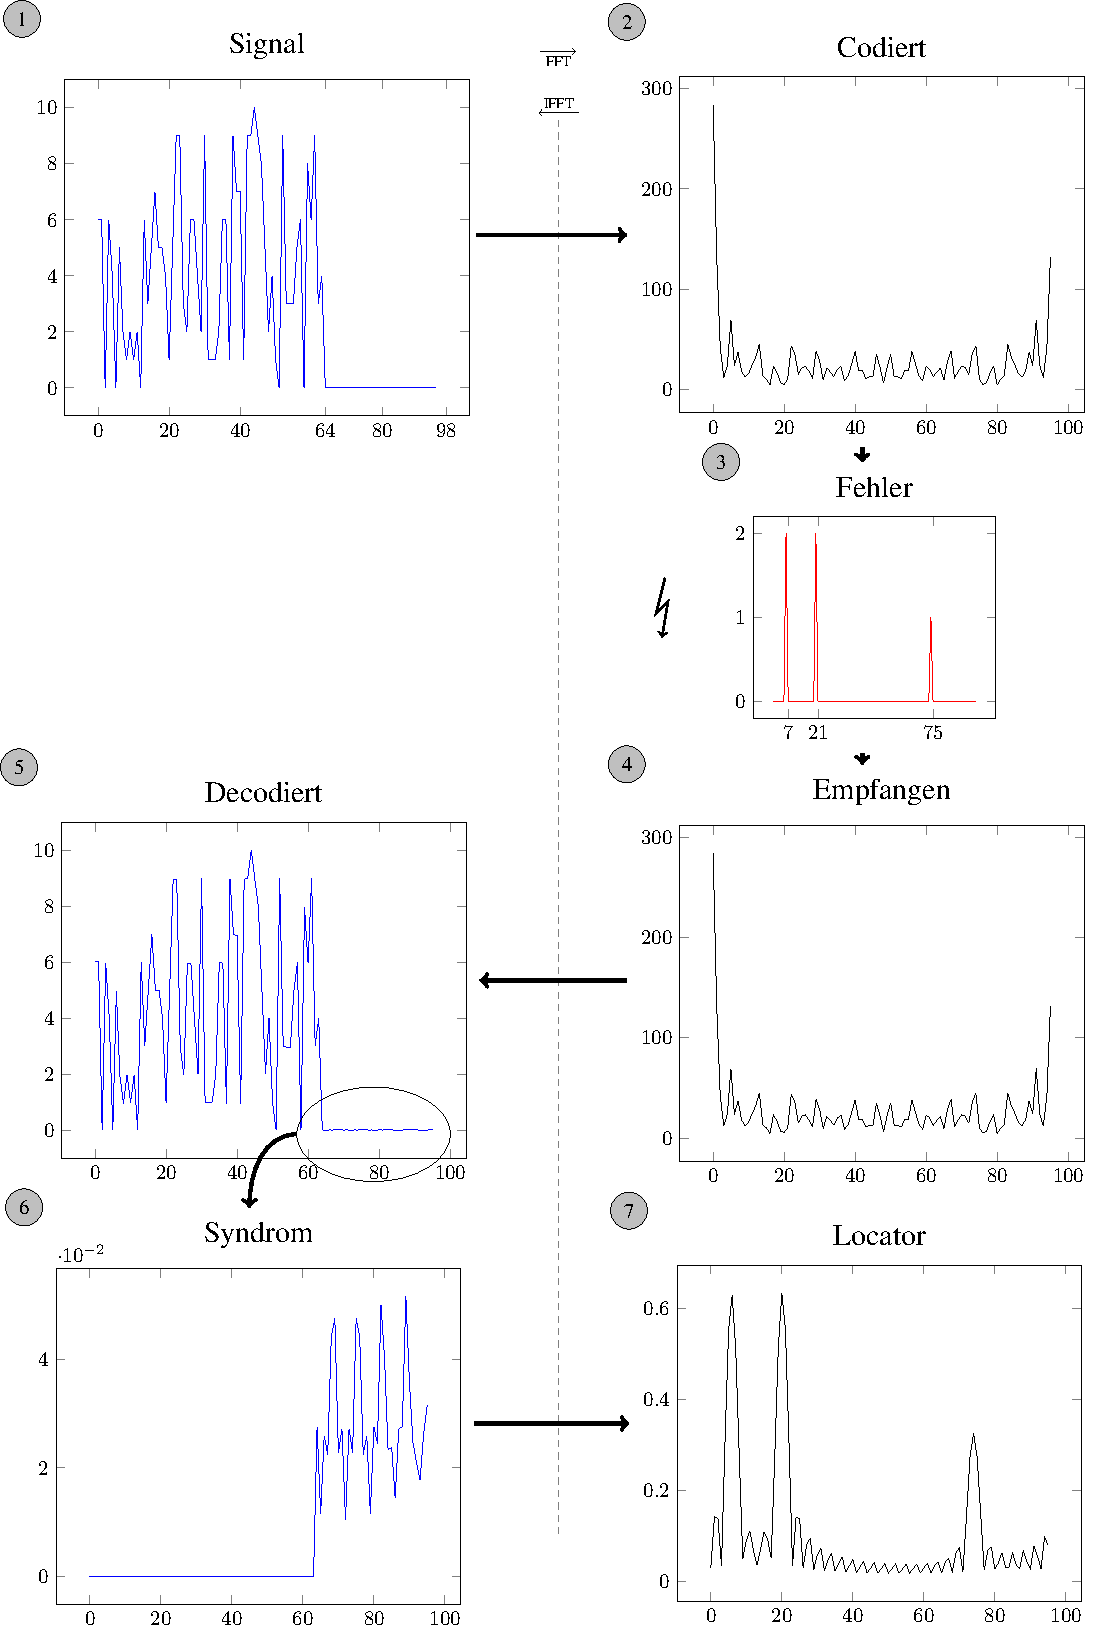
\includegraphics[width=\textwidth]{papers/reedsolomon/figures/plotfft}
    %%
% Plot der Übertrangungsabfolge ins FFT und zurück mit IFFT
%
\documentclass[tikz]{standalone}
\usepackage{amsmath}
\usepackage{times}
\usepackage{pgfplots}
\usepackage{pgfplotstable}
\usepackage{csvsimple}
\usepackage{filecontents}


\begin{document}
\begin{tikzpicture}[]

	%---------------------------------------------------------------
	%Knote
	\matrix(m) [draw = none, column sep=25mm, row sep=2mm]{

		\node(signal)  []    {
		\begin{tikzpicture}
			\begin{axis}
				[title = {\Large {Signal}}, 
				xtick={0,20,40,64,80,98}]
				\addplot[black] table[col sep=comma] {tikz/signal.txt};
			\end{axis}
		\end{tikzpicture}}; &
		
		\node(codiert) []    {
		\begin{tikzpicture}[]
			\begin{axis}[ title = {\Large {Codiert \space + \space Fehler}},
				xtick={0,40,60,100}, axis y line*=left]
				\addplot[green] table[col sep=comma] {tikz/codiert.txt};
			\end{axis}
			\begin{axis}[xtick={7,21,75}, axis y line*=right]
					\addplot[red] table[col sep=comma] {tikz/fehler.txt};
			\end{axis}
		\end{tikzpicture}}; \\
		
		\node(decodiert) []    {
		\begin{tikzpicture}
			\begin{axis}[title = {\Large {Decodiert}}]
				\addplot[blue] table[col sep=comma] {tikz/decodiert.txt};
			\end{axis}
		\end{tikzpicture}}; &
	
		\node(empfangen) []    {
		\begin{tikzpicture}
			\begin{axis}[title = {\Large {Empfangen}}]
				\addplot[green] table[col sep=comma] {tikz/empfangen.txt};
			\end{axis}
		\end{tikzpicture}};\\
	
		\node(syndrom) []   {
		\begin{tikzpicture}
			\begin{axis}[title = {\Large {Syndrom}}]
				\addplot[blue] table[col sep=comma] {tikz/syndrom.txt};
			\end{axis}
		\end{tikzpicture}}; &
	
		\node(locator) []    {
		\begin{tikzpicture}
			\begin{axis}[title = {\Large {Locator}}]
				\addplot[] table[col sep=comma] {tikz/locator.txt};
			\end{axis}
		\end{tikzpicture}};\\
	};
	%-------------------------------------------------------------
		%FFT & IFFT deskription
	
	\draw[thin,gray,dashed] (0,9) to (0,-9);
	\node(IFFT)  [scale=0.8]  at (0,9.3)   {IFFT};
	\draw[stealth-](IFFT.south west)--(IFFT.south east);
	\node(FFT)  [scale=0.8, above of=IFFT]    {FFT};
	\draw[-stealth](FFT.north west)--(FFT.north east);
	
	\draw[thick, ->,] (codiert)++(-1,0) +(0.05,0.5) -- +(-0.1,-0.1) -- +(0.1,0.1) -- +(0,-0.5);
	%Arrows
	\draw[thick, ->] (signal.east) to (codiert.west);
	\draw[thick, ->] (codiert.south) to (empfangen.north);
	\draw[thick, ->] (empfangen.west) to (decodiert.east);
	\draw[thick, ->] (syndrom.east) to (locator.west);
	\draw[thick](decodiert.south east)++(-1.8,1)  ellipse (1.3cm and 0.8cm) ++(-1.3,0) coordinate(zoom) ;
	\draw[thick, ->] (zoom) to[out=180, in=90] (syndrom.north);
	
	%item
	\node[circle, draw, fill =lightgray] at (signal.north west) {1};
	\node[circle, draw, fill =lightgray] at (codiert.north west) {2+3};
	\node[circle, draw, fill =lightgray] at (empfangen.north west) {4};
	\node[circle, draw, fill =lightgray] at (decodiert.north west) {5};
	\node[circle, draw, fill =lightgray] at (syndrom.north west) {6};
	\node[circle, draw, fill =lightgray] at (locator.north west) {7};
\end{tikzpicture}	
\end{document}
	}
	\caption{Übertragungsabfolge \ref{reedsolomon:subsection:Übertragungsabfolge}}
	\label{fig:sendorder}
\end{figure}